\begin{figure}[!htb]
\centering
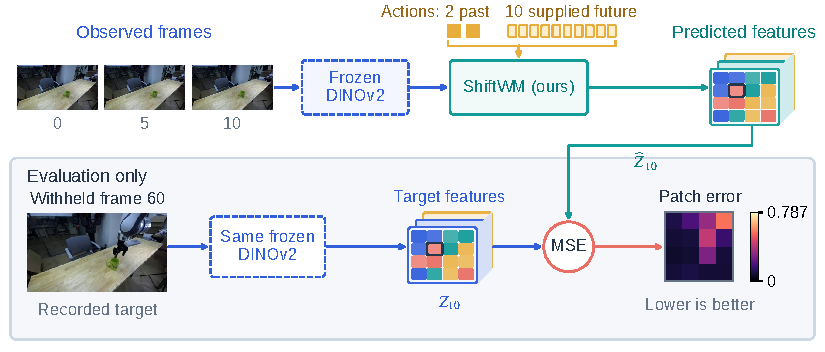
\includegraphics[width=\linewidth]{generated/editorial/task_story.pdf}
\caption[Recorded inputs and evaluator-only target.]{\textbf{Recorded inputs, predicted features, withheld evaluation.} Three observed frames (source indices 0, 5, 10), two past action blocks and ten supplied future blocks determine the feature forecast. Frame 60 enters only the evaluator through the same frozen DINOv2 encoder. Each block spans five source-frame intervals, not seconds. Layered feature objects are schematic; the heatmap is the actual three-seed, training-standardized $h=10$ patch MSE for the prespecified median-by-episode-gain case's first window (mean 0.1727; gain $-0.305\%$ versus autoregression), with the unchanged linear 0--0.787 scale. Recorded DROID images are unchanged (CC BY 4.0). Neither future RGB nor robot actions are generated.}
\label{fig:spatial-task}
\end{figure}
